\usepackage{longtable}\section{AFAPE}
\paragraph{AFA bootstrapping estimates for total costs}
\begin{figure}\centering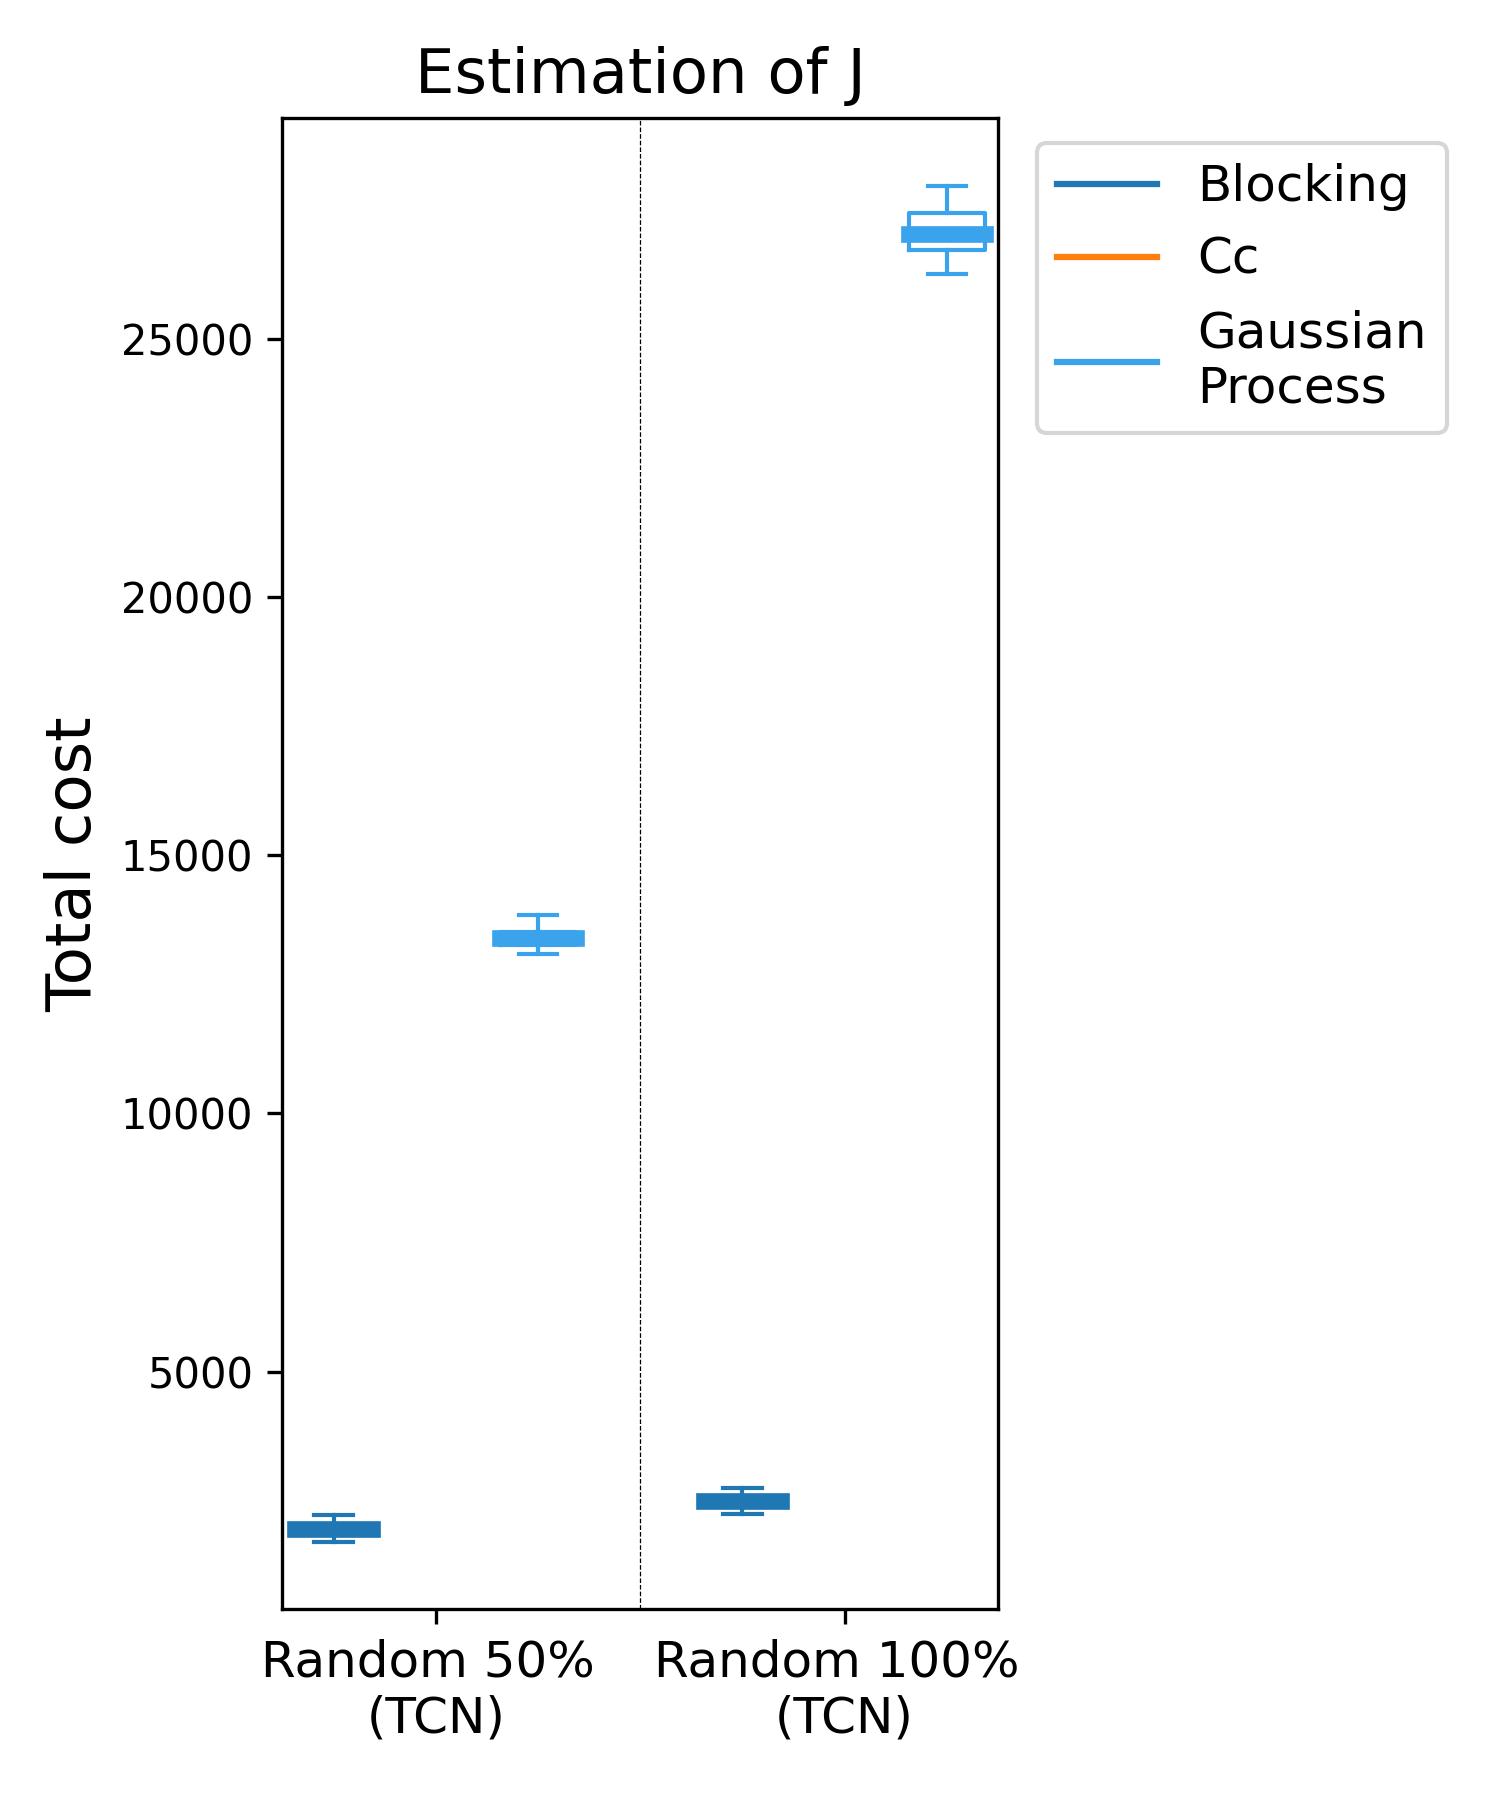
\includegraphics[width=0.5 \textwidth]{img/afape_report_afape_results_total.png}\caption{AFAPE for total cost for dataset miiv_10000_samples and missingness scenario MCAR_1}\label{fig:img/afape_report_afape_results_total.png}\end{figure}For individual\subparagraph{AFAPE for total cost for agent Random 50% (TCN)}
\begin{longtable}{lr}
\hline
 Estimator        &   Estimate \\
\hline
\endhead
 Blocking         &    1948.37 \\
 CC               &     nan    \\
 gaussian\_process &   13413.6  \\
\hline
\end{longtable}For individual\subparagraph{AFAPE for total cost for agent Random 100% (TCN)}
\begin{longtable}{lr}
\hline
 Estimator        &   Estimate \\
\hline
\endhead
 Blocking         &    2495.17 \\
 CC               &     nan    \\
 gaussian\_process &   27088.4  \\
\hline
\end{longtable}